\documentclass{article}
\usepackage[T1]{fontenc}
\usepackage{lmodern}
\usepackage{graphicx}
\usepackage{amsmath,amssymb}
\usepackage[a4paper,margin=2cm]{geometry}
\usepackage[absolute,overlay]{textpos}
\setlength{\TPHorizModule}{1mm}
\setlength{\TPVertModule}{1mm}
\usepackage[indonesian]{babel}
\usepackage{hyperref}
\setlength{\emergencystretch}{2em}
% unit: Halaman 5

\begin{document}

% === Halaman 5 (python/native) ===

Rinaldi M/II4020 Kriptografi

5

Sumber: https://www.mayurpahwa.com/2018/12/hybrid-cryptography.html 

Hybrid Cryptography

K

PKBob

SKBob

K

% deskripsi: gambar native xref 33
\noindent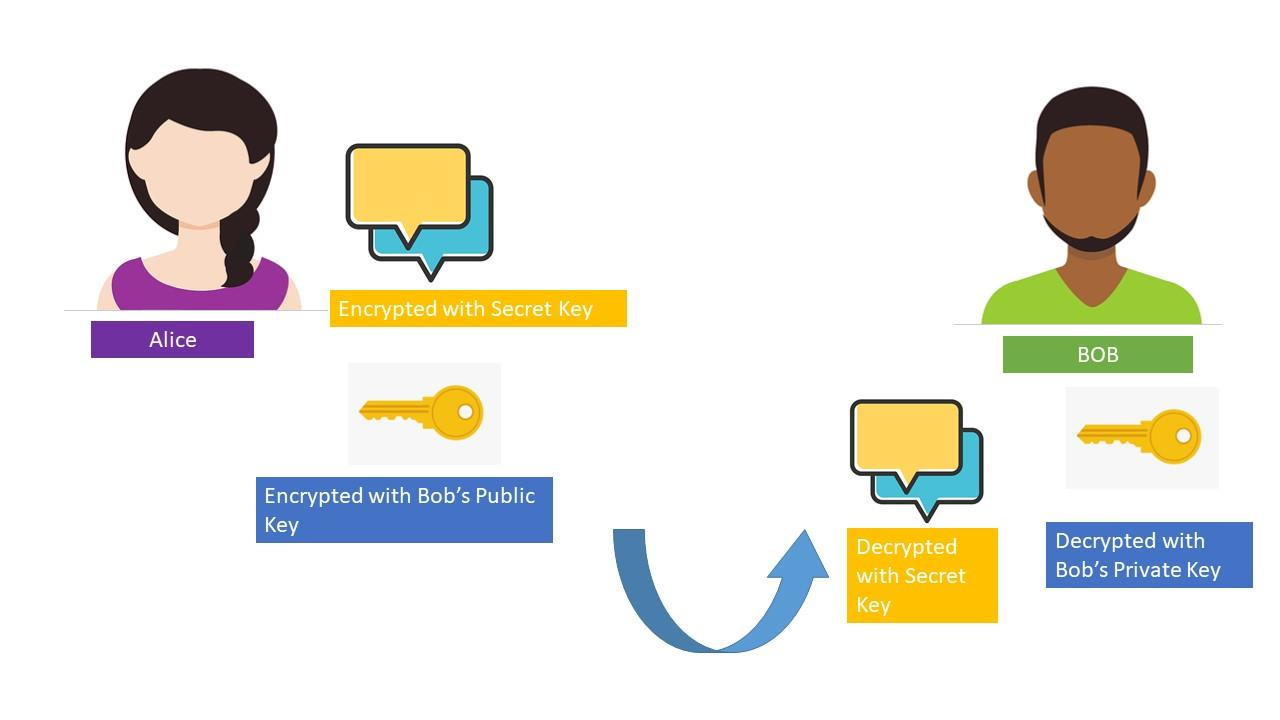
\includegraphics[width=0.85\textwidth]{../../images/python/page_005_img_01.jpeg}

\end{document}
